\chapter{Tutorial}
In this chapter, you will learn the basic operation of a test board setup, communication with the test board and a single chip.

%---------------------------------------------------------------------
\section{Requirements}
To work yourself through this tutorial, you need
\begin{itemize}
    \item A DTB, connected to your computer via USB
    \item An adapter board for a single chip
    \item A single chip holder, equiped with a chip (does not require a sensor)
    \item The software \texttt{psi46test} installed
    \item An oscilloscope, fast enough to resolve 200\,MHz signals
    \item NIM cables of equal length (i.e.\, 6\,ns delay or similar)
\end{itemize}
\todo{Find conistent names for the adapter card and the single chip card and use it consistently.}

\todo{Check this list and adjust requirements if needed}

If you need help to set this up, please go to the \enquote{How To's} in chapter \ref{sec:howto}.

\note{Whenever you do any change to the testboard (i.e.~switch adapter cards, switch chips etc.), make sure that the chip is not powered. To do so, check that the red LED labeled \enquote{RUN} is dark. If not, issue the command \psicommand{poff} from within \texttt{psi46test}. When you insert a chip holder, make sure you, the testboard and the chip holder are properly grounded before insertion.}

%---------------------------------------------------------------------
\section{Hello world}

\todo{First try out welcome command}

%A first test is to see if supply voltages are present. Invoke \texttt{psi46test} and issue the command

A basic test is to see if we can trigger on a signal and see something. For this test, connect an adapter card to the DTB but do not insert a chip holder. We program the built-in pulse generator to send a sync signal and a token. The sync signal is not routed to the chip. It is only used as a marker of the pulse sequence so that the oscilloscope has a meaningful signal to trigger the scope on. The token is a signal that would be passed to the \gls{ROC}, if one is connected.

Make the following connections:
\begin{itemize}
    \item Connect the \enquote{D1} output of the DTB to the first channel of your scope
    \item Connect the \enquote{A1+} output of the DTB to the second channel of your scope
\end{itemize}
Then issue the following sequence from within \texttt{psi46test}:

\bigskip

\begin{tabular}{lp{0.6\textwidth}}
    \toprule
Command & Brief description \\
    \midrule
\psicommand{pon}               & Turn on the testboard power \\
\psicommand{d1 \vuse{dsp:val:pg_sync}} & This selects pg\_sync as signal routed to D1\\
\psicommand{a1 \vuse{asp:val:TIN}}     & Select the token in signal as analog signal routed to A1\\
\psicommand{pgset 0 b100001 0} & Program the pulse generator to send a sync and a token out \\
\psicommand{pgloop 1000}       & Start the pulse generator. Repeats the pulse sequence infinitely, start a new cycle every 1000 clock cycles\\
    \midrule
\psicommand{poff}              & Turn off the testboard power. Do this after you are finished with your measurements. \\
    \bottomrule
\end{tabular}

\bigskip

Here, one clock cycle is 25\,ns long, i.e.~the frequency is 40\,MHz, which is the same as the LHC collision frequency.

Set up your scope to continuously trigger on the first channel (D1) and you should see something like what is shown in Fig.~\ref{fig:tut_scope1}. In case you cannot reproduce this, check your setup for mistakes and inspect the settings on your scope.
\begin{figure}[h]
    \begin{center}
	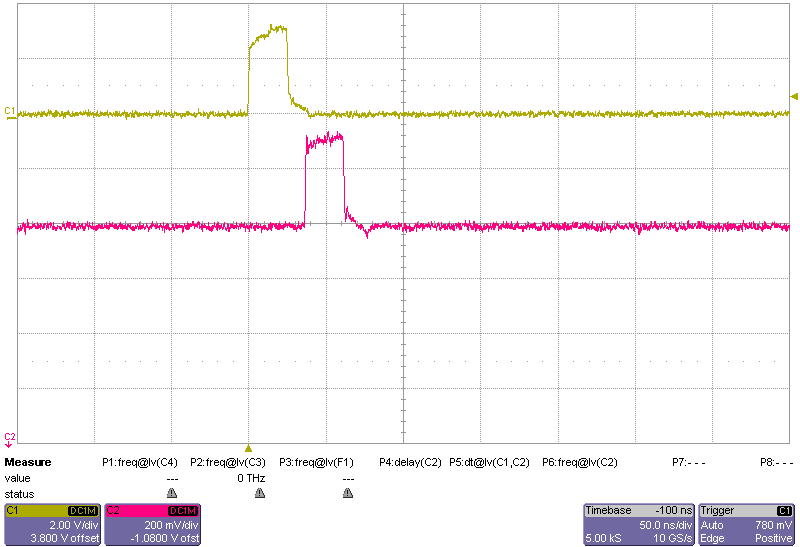
\includegraphics[width=0.7\textwidth]{img/tut_scope1.png}
	\caption{Output of the \enquote{hello world} test. The first channel (yellow, top) shows the sync signal. It has a width of 25\,ns. The second signal is the token (magenta). It appears with some delay and has the same width.}
	\label{fig:tut_scope1}
    \end{center}
\end{figure}

Now let us see what this sequence actually does.  The first two steps select the signals of the digital and analog outputs that are routed to the scope. The \psicommand{pgset} is used to define a pattern that will be generated every 1000 clock cycles again. Zoom out in the time domain and at a point you should see the signal from the following cycle. Reduce the number of cycles in \psicommand{pgloop} if necessary.

The pattern we use here consists of just one set of bits set at the begin of the cycle. This command is more powerful, as we will see later on. Here, we only ask the pulse generator to send a sync and a token out signal at the begin of the cycle and nothing else follows. The meaning of the terminating 0 in \psicommand{pgset 0 b100001 0} is that no other signal will follow.
%You can think of such a sequence as a small program. Using the command \psicommand{pgset} one can create pulse sequences to test different things. Our sequence has only one step where we create a pulse on the sync and the token signal. One step has a number, a bit pattern and a delay to the next pattern. If the delay is set to 0, the cycle ends, as it does in our example. The bit pattern is given as a binary number, starting with a \psicommand{p}. The following bits can be set:
\begin{center}
\begin{tabular}{lcccccc}
    \toprule
Bit:  & 0 & 1 & 2 & 3 & 4 & 5 \\
Name: & sync & reset TBM & reset ROC & calibrate & trigger & token \\
Abbreviated name: & (sync) & (rest) & (resr) & (cal) & (trg) & (tok) \\
    \bottomrule
\end{tabular}
\end{center}

We see what we expect: a sync and a token signal, as we observed. So we understand what the sequence does. And we know that our setup works.
\todo{Explain the delay between the two signals.}

% px4.png


%---------------------------------------------------------------------
\section{Basic communication with a ROC}

Now we insert a \gls{ROC} into the adapter board. Don't forget to check that nothing is running and all LED's are dark before inserting the chip. Make sure that you insert the chip card the right way, i.e.~the wirebonds should face towards the DTB.

Add another cable to connect \psicommand{A2+} to the third channel of your scope.

We want to see the \gls{ROC} talking. For this we simply send a command to the chip and see what happens. For the moment it doesn't matter what we send out, sending \psicommand{cald} does the job. This command deletes all calibrate settings in the chip and is the only command which takes no parameter. So the sequence of commands in \texttt{psi46test} is:

\bigskip

\begin{tabular}{lp{0.6\textwidth}}
    \toprule
Command & Brief description \\
    \midrule
\psicommand{pon}   & Turn on the testboard power \\
\psicommand{clk 0} & Resets some timing parameter \\
\psicommand{ctr 0} & Resets some timing parameter \\
\psicommand{sda 0} & Resets some timing parameter \\
\psicommand{tin 0} & Resets some timing parameter \\
\psicommand{select 0} & Sets the address of the chip we want to talk to \\
\psicommand{d1 \vuse{dsp:val:send}}  & Select the \psicommand{send} signal as the one we trigger on the scope \\
\psicommand{a1 \vuse{asp:val:CLK}}  & Select the clock signal for channel 2 \\
\psicommand{a2 \vuse{asp:val:SDA}}  & Select the send data signal for channel 3 \\
\psicommand{cald}  & Program a register on the ROC \\
    \midrule
\psicommand{poff}              & Turn off the testboard power. Do this after you are finished with your measurements. \\
    \bottomrule
\end{tabular}

\bigskip

The four timing parameters we just set to a default value of 0. We will adjust them in the next part of this tutorial.
To make things visible you need to use the scope in single trigger mode. You can issue the \psicommand{cald} command as often as you want. You should see something like in Fig.~\ref{fig:tut_scope2}.

\begin{figure}[h]
    \begin{center}
	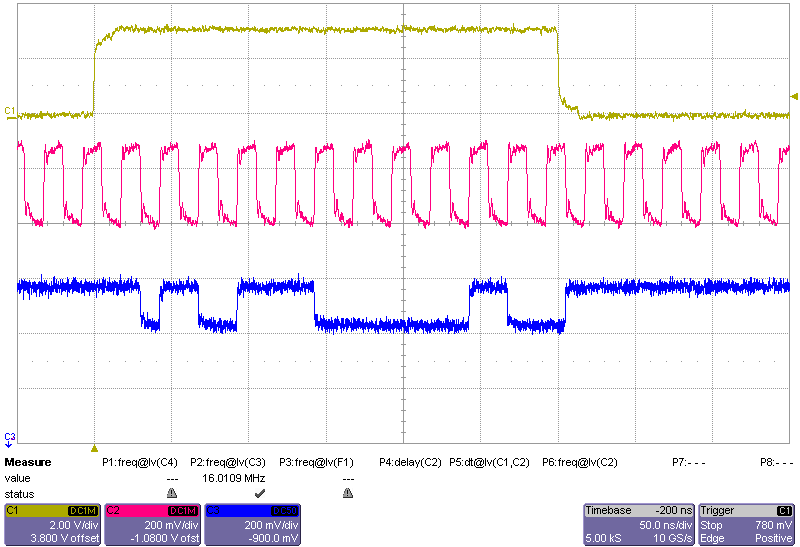
\includegraphics[width=0.7\textwidth]{img/tut_scope2.png}
	\caption{Simple communication to the \gls{ROC}. The first signal (yellow) shows the signal we trigger on, the \psicommand{send} signal. The second signal (magenta) is the clock and the third (cyan) the signal sent to the \gls{ROC}. Observe that the timing of the signals are not yet correct.}
	\label{fig:tut_scope2}
    \end{center}
\end{figure}

The result shows the signal we trigger on. The \psicommand{send} signal is internal to the testboard and only available to our convenience for triggering. The clock is here to give an idea over what timeframe the action happens and as a reference frame for the timing. The activity spans over several clock cycles. It begins with the header addressing the \gls{ROC}, followed by a bunch of other signals in a pattern we do not need to understand right now. In our example we did not set a specific \gls{ROC} address (the value to talk to a specific \gls{ROC}). If we would work with a module, 16 \gls{ROC}'s would be present. With this address we would choose to which of these we want to talk. The default value is \psicommand{0}. But how is this encoded? To address one \gls{ROC} out of 16 we need four bits. Encoding 0 would end in \psicommand{b0000}. So we should see four zeroes, which is what we see. The length of one bit is a full clock cycle, i.e.~clock up and down. Try to count the clock cycles and make sure you understand how this works.

You can change the \gls{ROC} address to talk to by issuing \psicommand{select N}, where N is a number between 0 and 15 and see what changes. If you do e.g.~\psicommand{select b0111} (recall: a number starting with a b is interpreted as a binary number, which comes in handy here) then you see that the signal is low for a logical 0 and then three logical 1 follow. Play around with different numbers to make sure you understand this pattern.

\section{Listening to the ROC}
The result of the previous step shows the testboard talking to the \gls{ROC} only. The real thing is to talk to the \gls{ROC} and read back some information. But for this we need to work on some timing issues first. The \gls{ROC} receives signals in an encoded form, as we have seen in the example above. The clock is used as the reference to synchronize all signals to.

What we will do first is to adjust the timing of signal to program the \gls{ROC} relative to the clock. For this we use the same setup as before and start to set values for the delay of the clock signal \psicommand{clk} and the send data signal \psicommand{sda}. All delay values can be set as positive numbers up to a maximum of about 300. One unit corresponds to $1/20$ of a clock cycle. So setting a value of 20 would shift the delay by exactly one clock cycle. Issue the following command and see what happens:

\bigskip

\begin{tabular}{lp{0.6\textwidth}}
    \toprule
\psicommand{clk 20} & Sets the delay of the clock to 20, i.e.~one full cycle \\
    \bottomrule
\end{tabular}

\bigskip

As expected, you see no significant change. The clock has been shifted by one full cycle, so the picture should be the same.

Observe that we no longer write \psicommand{pon} and \psicommand{poff} at the begin and end of the sequence. Make sure you do this whenever you measure something.

We can only set positive values. At some point we might want to have the ability to set delays negative to the clock. Therefore we set the value to some positive number, say 10:

\bigskip

\begin{tabular}{lp{0.6\textwidth}}
    \toprule
\psicommand{clk 10} & Sets the delay of the clock to 10, i.e.~one half cycle \\
    \bottomrule
\end{tabular}

\bigskip

The change you see on the oscilloscope is minimal. The clock is shifted by half a cycle, so more or less inverted. Now we need to know how we have to set the \psicommand{sda} signal relative to the clock. The programming of the chip uses a modified \isqc{} signal. Modified means here that not the full set of possibilities are implemented. \isqc{} is an industry standard to communicate with electronic devices and is widely used for example in the car industry. Our implementation differs that we can send data much faster but cannot read back on the same wire.

\isqc{} is a serial interface and uses a clock and a data wire to communicate. The following states are possible:

\bigskip

\begin{tabular}{lcl}
    \toprule
Name & Data signal while clock is high & Description \\
    \midrule
idle & high & No data transferred \\
start & falling edge & Data transfer starts \\
data & high or low & Data to be transferred \\
stop & rising edge & Data transfer ends \\
    \bottomrule
\end{tabular}

\bigskip

All the interesting stuff goes on when clock is on high level. Before we try to analyse the signal in detail we adjust the timing. The very first change on \psicommand{sda} should be a drop from high to low while clock is high (start). So inspecting Fig.~\ref{fig:tut_scope2} shows that this is not the case. Try to shift the signal by setting the delay using the \psicommand{sda} command to the smallest possible value but not smaller than what we used for \psicommand{clk}. You should end up with something that looks like Fig.~\ref{fig:tut_scope3}

%\begin{figure}[h]
%    \begin{center}
%	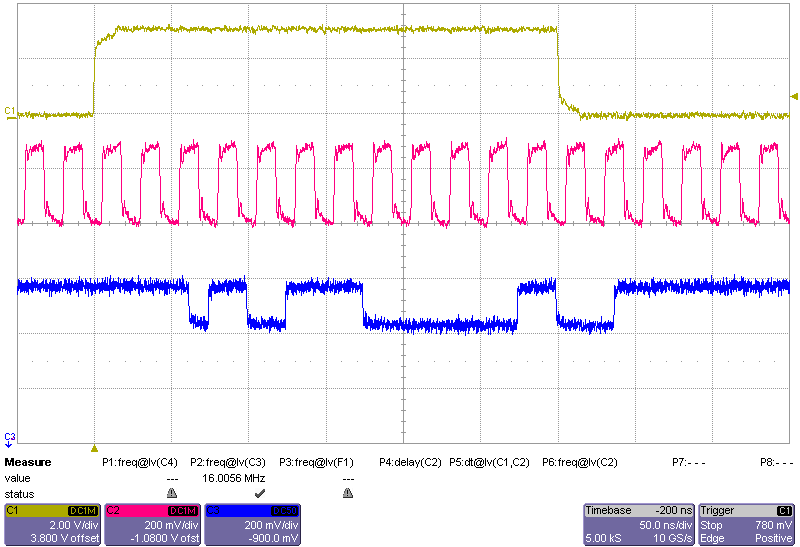
\includegraphics[width=0.7\textwidth]{img/tut_scope3.png}
%	\caption{Same as in Fig.~\ref{fig:tut_scope2} but now the timing is correctly adjusted between clock and send data.}
%	\label{fig:tut_scope3}
%    \end{center}
%\end{figure}

\begin{figure}[h]
    \begin{center}
	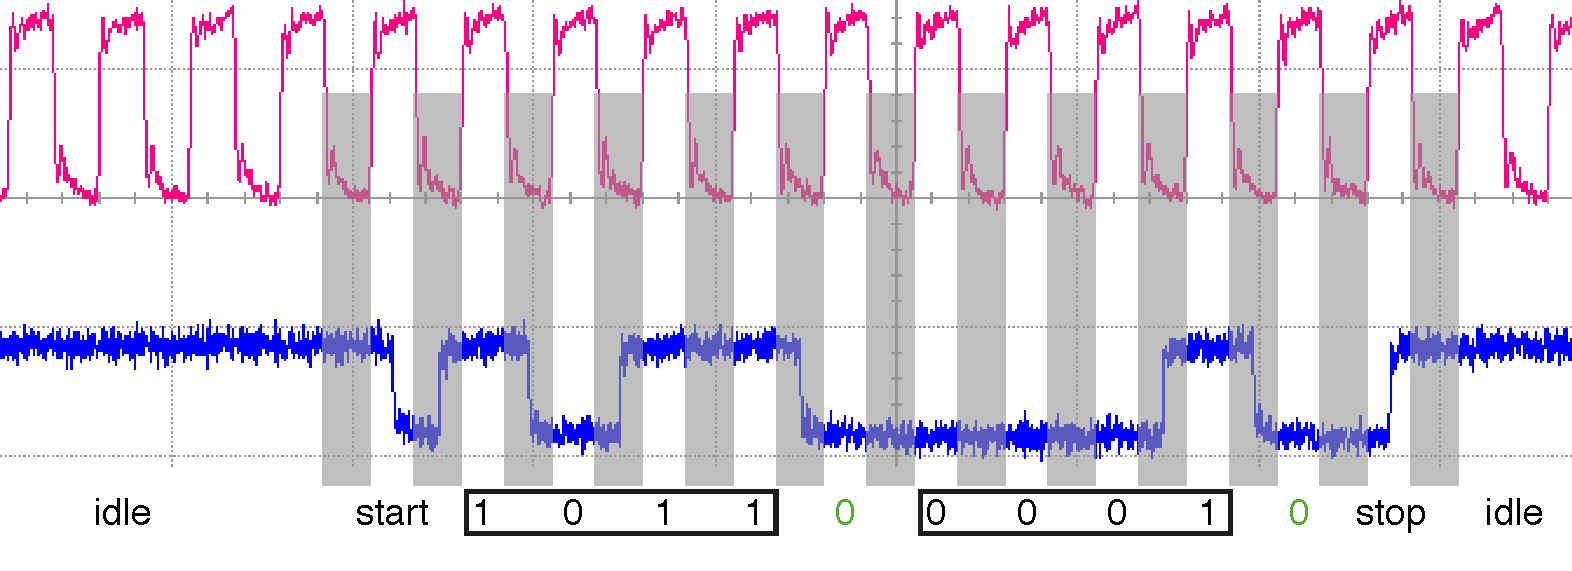
\includegraphics[width=0.7\textwidth]{img/tut_scope3_crop.pdf}
	\caption{Detail of Fig.~\ref{fig:tut_scope3}. The times when clock is high are clear and when clock is down has been greyed out. Recall that in this protocol the signal is only meaningful when clock is high. The idling time is interrupted by a start signal, followed by the data 10110001. Then the stop signal appears and the idle signal appears again. The function of the additional zero (in green) is explained in the text.}
	\label{fig:tut_scope3}
    \end{center}
\end{figure}

Now we want to understand what is going on. Fig.~\ref{fig:tut_scope3} shows the relevant section. Let's see if we can identify all stages of the transmission. It first starts with a long idle section. Then the communication starts. While clock is high the signal edge transitions to low. All the following data is either 0 or 1 and is constant while clock is high. Then the signal edge rises while clock is high, the data transmission has ended and returns to idle. The data is arranged in groups of 5 bits. The first four are the data bits and the fifth is bit number~4 inverted. So if the data is e.g.~1001, then the fifth bit would be 0. The full group would be 10010. And if the data is 1000 then the full group would be 10001. The reason for this is to make sure that the signal is more balanced in 0 and 1. In CMS the data would be transferred to an optical transmission line. The receiver at the end of it has an auto-gain feature which would increase the amplification if nothing happens for some time. Would a data transfer consist of a lot of zeroes, the signal would look constant for a while. This trick with adding a fifth inverted bit does the trick. 00000000 would end up as 0000100001.

So what does this transmitted data mean? The first group of four is the ROC address. In this case we used \psicommand{b1011} as address, so this is what we find. Adjust your \psicommand{select} command to select b1011 if you want to see exactly the same output. The second group of four bits is the command. The possibilities are:

\bigskip

\begin{tabular}{clll}
    \toprule
    Code & Meaning & Following parameters & Total length \\
    \midrule
    1000 & dac programming (setdac)    & 2$\times$8\,bits & 20\,bits \\
    0100 & pixel programming           & 3$\times$8\,bits & 28\,bits \\
    0010 & calibration set             & 3$\times$8\,bits & 28\,bits \\
    0001 & calibration delete (cald) & no parameters & 4\,bits \\
    \bottomrule
\end{tabular}

\bigskip

Intentionally we sent the simplest command we can, \psicommand{cald}. So we expect just the four command bits 0001 and nothing else, as \psicommand{cald} takes no parameter.

Now let's see if this actually works, i.e.~if the \gls{ROC} receives a command and acts upon. First, we need to make sure that the \gls{ROC} has the right address. Set its address to the same value as you used in te last \psicommand{select} command, i.e.~do \psicommand{rocaddr b1011}. This command works only in the case of a single \gls{ROC}, as we do it now. It gives the \gls{ROC} the specific address. In a module, a \gls{ROC} gets its address via some hard-wired signals between the \gls{ROC} and the \gls{HDI} circuit. In our setup we do not have an \gls{HDI}, so some logic in the testboard emulates the function of a \gls{TBM} and we can tell this logic which address it should assign to the \gls{ROC}. To talk to it, the value after \psicommand{select} needs to match.

We just set up the sending of commands. We are not yet capable of reading back from the \gls{ROC}. But we can see if the \gls{ROC} reacts to commands we send to it. \psicommand{getia} displays the current analog current. Try it out. It should be close to zero. Now send a command to the chip which should make him to draw some current. Setting the analog voltage in the chip, $V_\text{ana}$, will do the trick. Set $V_\text{ana}$ to some value, say \psicommand{vana 100} and check the current again. It should be higher. The \gls{ROC} actually received a command and we can see that something happens.

\section{Reading from the ROC}

\bigskip

\begin{tabular}{lp{0.6\textwidth}}
    \toprule
Command & Brief description \\
    \midrule
\psicommand{pon}   & Turn on the testboard power \\
\psicommand{clk 10} & Resets some timing parameter \\
\psicommand{sda 25} & Resets some timing parameter \\
\psicommand{ctr 10} & Resets some timing parameter \\
\psicommand{tin 15} & Resets some timing parameter \\
\psicommand{pgset 0 b101000 10} & \\
\psicommand{pgset 1 b000100 40} & \\
\psicommand{pgset 2 b000010 16} & \\
\psicommand{pgset 3 b000001 0} & \\
\psicommand{rocaddr b1011} & Sets the address of the chip \\
\psicommand{select b1011} & Sets the address of the chip we want to talk to \\
\psicommand{d1 9}  & \\
\psicommand{a1 0}  & \\
\psicommand{a2 1}  & \\
\psicommand{pgloop 1000}  & \\
    \bottomrule
\end{tabular}

\bigskip

\todo{Mention that we have a differential signal. Might be good to hook up A2- and calculate the difference}


\bigskip

\begin{tabular}{lp{0.6\textwidth}}
    \toprule
Command & Brief description \\
    \midrule
\psicommand{vcal 60}   & \\
\psicommand{vthr 60}   & \\
\psicommand{wbc 40}   & (needs a scan) \\
\psicommand{cole :}   & \\
\psicommand{pixe 10 10 0}   & \\
\psicommand{cal 10 10}   & \\
    \bottomrule
\end{tabular}

\bigskip

